% vim: set tw=78 aw:
\documentclass{beamer}

\usepackage[utf8x]{inputenc}
\usepackage[romanian]{babel}
\usepackage{hyperref}
\usepackage{graphicx}
\usepackage{comment}
\usepackage{tikz}
\mode<presentation>
{ \usetheme{Rochester} }

\title{Profiling}
\subtitle{Prezentare ROSEdu Tech Talks}
\institute{ROSEdu}
\author{Vlad Dogaru \texttt{ddvlad@rosedu.org}}

\begin{document}

\frame{\titlepage}

\section{Why profiling?}

\frame{\tableofcontents[currentsection]}

\begin{frame}{So what the heck is profiling anyway?}
  Profiler = utilitar pentru analiza \textit{dinamică} a programelor
  \begin{itemize}
    \item analiza performanțelor
    \item analiza memoriei
    \item simularea unui întreg set de instrucțiuni
  \end{itemize}
\end{frame}

\begin{frame}{Tipuri de profilere}
  După formatul output-ului:
  \begin{itemize}
    \item flat profiling
    \item call graph profiling
  \end{itemize}
  \pause
  După metoda de obținere a datelor:
  \begin{itemize}
    \item event based
    \item statistical
    \item instrumenting
  \end{itemize}
\end{frame}

\section{gprof}
\frame{\tableofcontents[currentsection]}

\begin{frame}{gprof}
  \begin{itemize}
    \item parte a GNU binutils
    \item generează atât date \textit{flat}, cât și \textit{call-graph}
    \item necesită instrumentarea programelor la compilare și link-editare
    (pentru partea de call-graph)
    \item folosește sampling pentru informații de timing
  \end{itemize}
\end{frame}

\begin{frame}{gprof -- The Magick}
  \begin{center}
    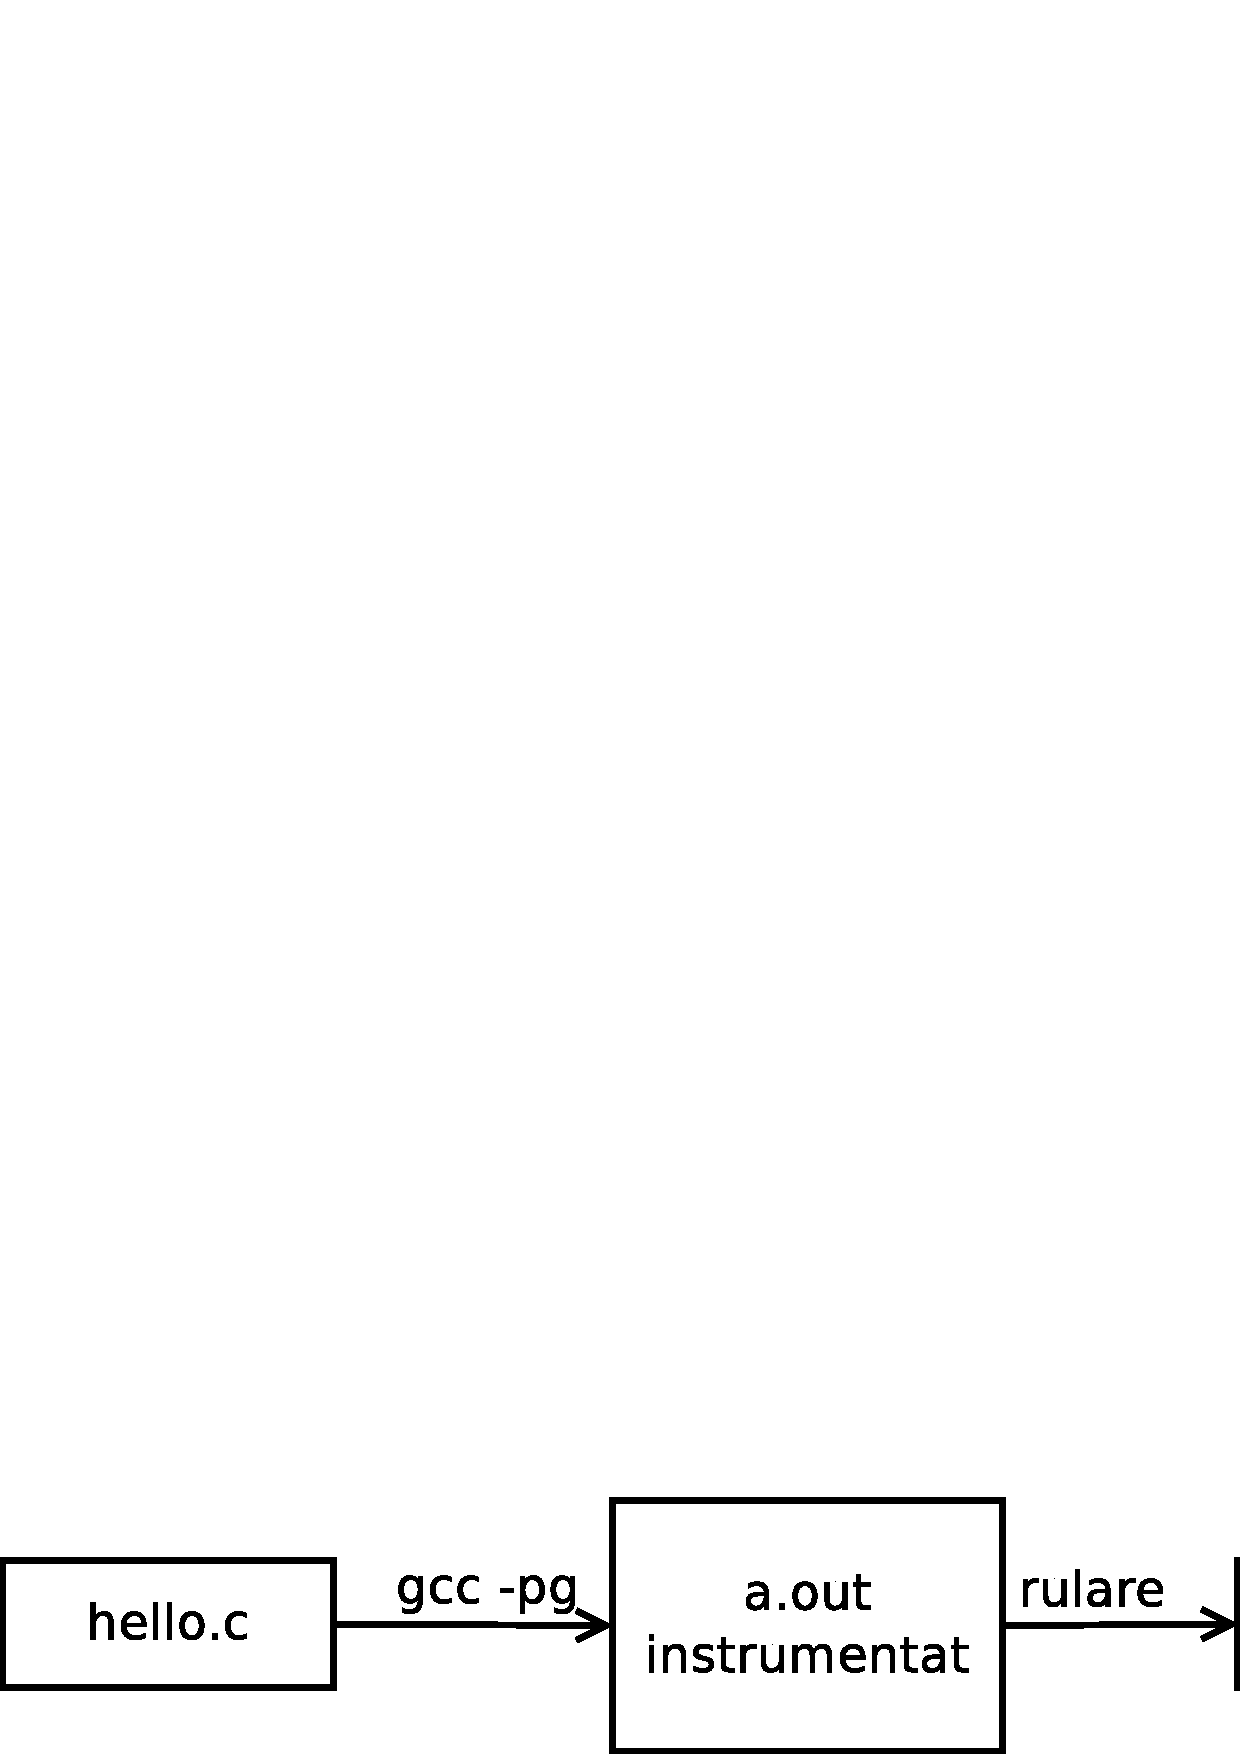
\includegraphics[width=0.8\textwidth]{gprof.pdf}
  \end{center}
\end{frame}

\begin{frame}{gprof Hands-On}
  \begin{itemize}
    \item compilare și link-editare cu \texttt{-pg}

    \begin{beamerboxesrounded}[lower=block
    body,shadow=true,width=0.7\textwidth]{}
      \texttt{CFLAGS += -pg}
    \end{beamerboxesrounded}
    \item rulare program -- este generat fișierul \texttt{gmon.out}
    \item rulare gprof:

    \begin{beamerboxesrounded}[lower=block
    body,shadow=true,width=0.7\textwidth]{}
      \texttt{\$ gprof executabil gmon.out}
    \end{beamerboxesrounded}
    \item implicit, gprof generează ambele tipuri de analiză
  \end{itemize}
\end{frame}

\begin{frame}{Live Demo}
  \begin{itemize}
    \item Problema: se dau $n$ matrice pătratice. Să se decidă dacă prima are
    determinantul maxim.
    \pause
      \begin{itemize}
      \item da, e o problemă banală :-(
      \end{itemize}
  \end{itemize}
\end{frame}

\section{OProfile}
\frame{\tableofcontents[currentsection]}

\begin{frame}{OProfile -- How it works}
  \begin{itemize}
    \item sampling, folosind registre hardware (\textit{performance counters})
    \item la fiecare overflow al unui registru, se declanșează o întrerupere
    \item handler-ul de întrerupere actualizează statisticile
    \item la final, se generează un raport
  \end{itemize}
\end{frame}

\begin{frame}{OProfile -- Pros and Cons}
  Avantaje:
  \begin{itemize}
    \item analizează întreg sistemul
    \item overhead mic
    \item valoare de overflow configurabilă
    \pause
    \begin{itemize}
      \item valoare prea mică $\Rightarrow$ multe întreruperi $\Rightarrow$
      sistem ``pe butuci''
    \end{itemize}
    \pause
    \item întrerupere nemascabilă, deci putem analiza inclusiv kernelul
    \item gamă largă de criterii de analiză: cache hits, TLB hits, operații
    aritmetice
  \end{itemize}

  \pause
  Dezavantaje:
  \begin{itemize}
    \item analizează întreg sistemul
    \item necesită suport în kernel
    \item generează call graphs pe puține arhitecturi
    \item necesită acces \texttt{root} pe mașina gazdă
  \end{itemize}
\end{frame}

\begin{frame}{Oprofile -- Arhitectură}
  \begin{center}
    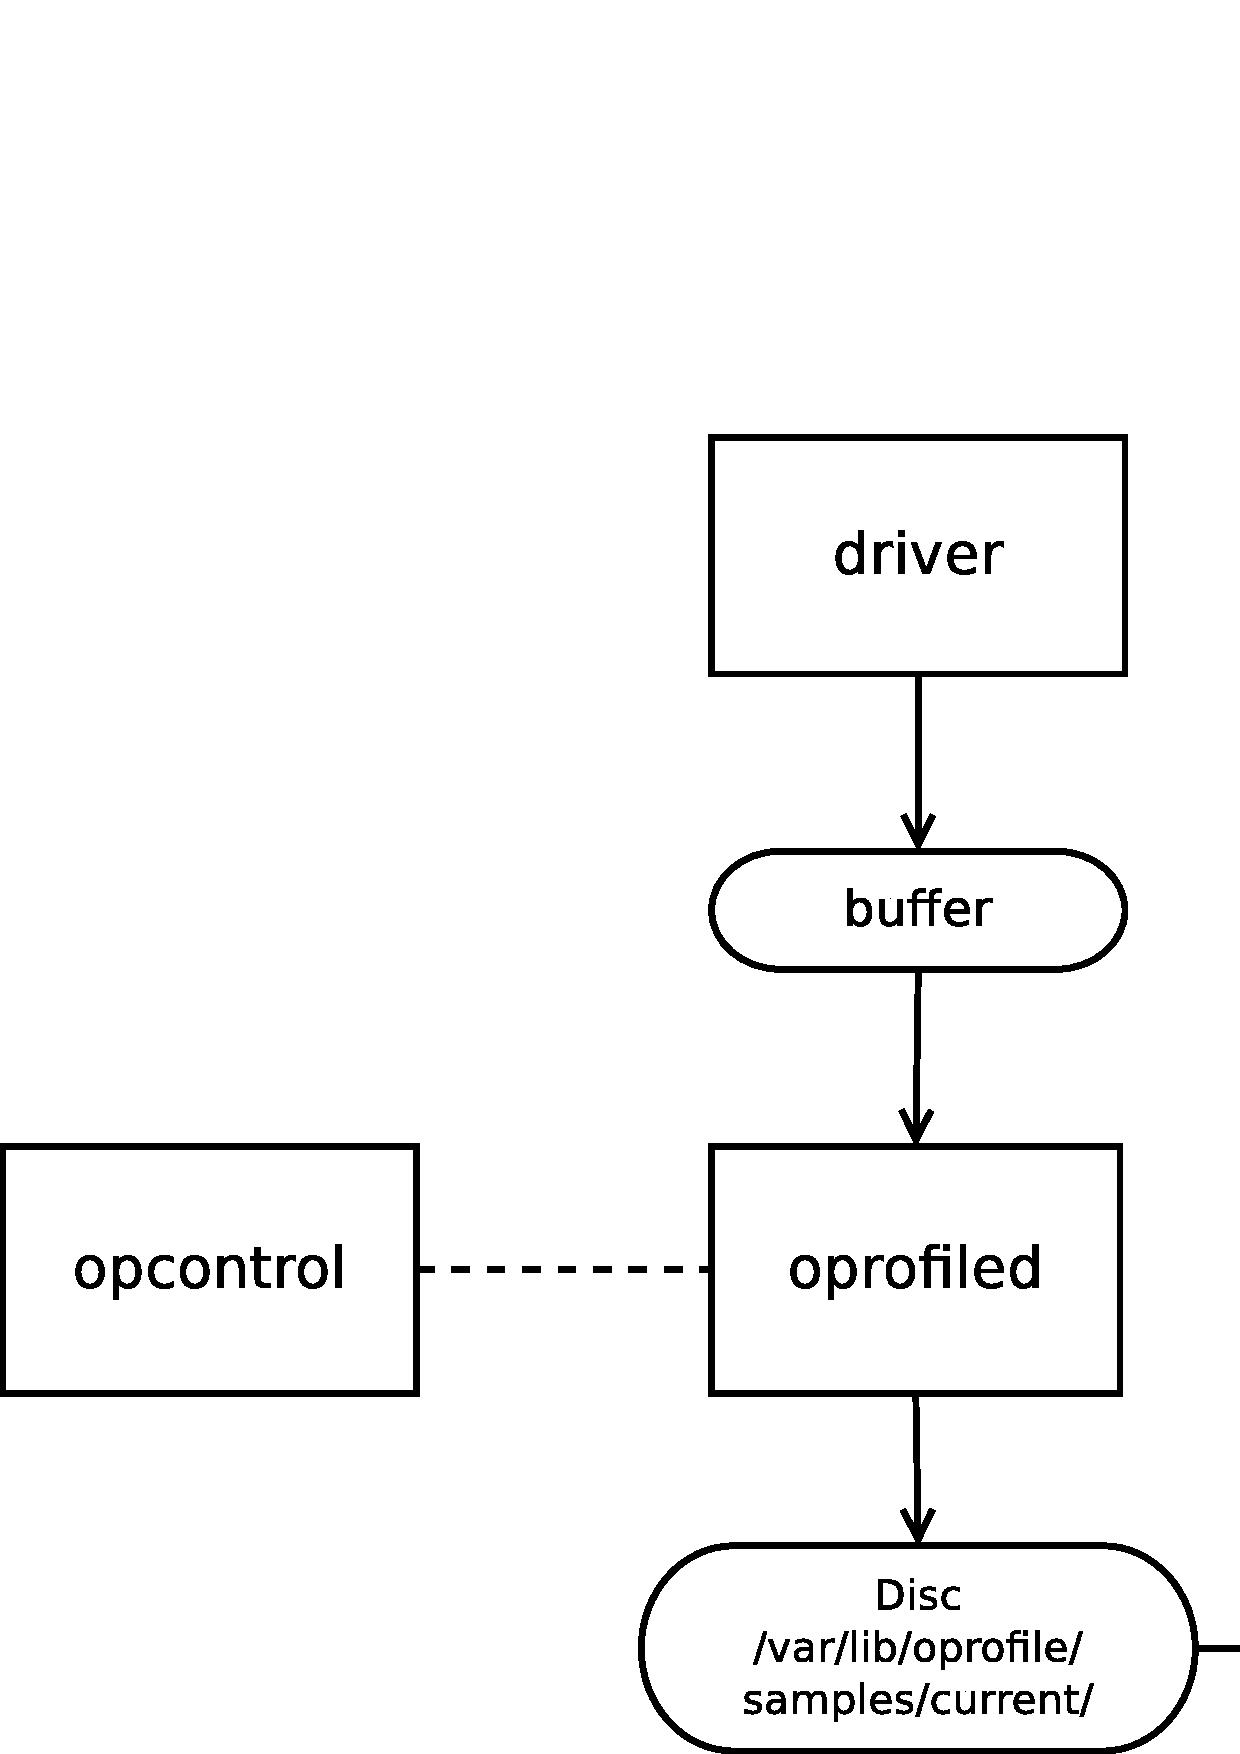
\includegraphics[width=0.6\textwidth]{oprofile.pdf}
  \end{center}
\end{frame}

\begin{frame}{4 Steps to Happiness}
  \begin{enumerate}
  \item Copilare kernel cu suport OProfile, instalare utilitar userspace
  \item Configurare și pornire profiler:

    \begin{beamerboxesrounded}[lower=block body,shadow=true]{}
      \texttt{\$ oprofile --vmlinux=/path/to/vmlinux \textbackslash} \\
      \qquad \qquad \texttt{-e L1I\_MISSES:1000}\\
    \end{beamerboxesrounded}
    \texttt{\$ oprofile --start}
  \item Rulare program de analizat
  \item Generarea unui raport

    \begin{beamerboxesrounded}[lower=block body,shadow=true]{}
      \texttt{\$ opreport -l \# Global} \\
      \texttt{\$ opreport -l /path/to/my/binary}
    \end{beamerboxesrounded}
  \end{enumerate}
\end{frame}

\begin{frame}{Exemplu}
  \begin{itemize}
    \item \textbf{Problema:} Numărăm toți multiplii de 2 și 3 mai mici decât
    $2^{30}$.
    \item Serial: \\
      \begin{beamerboxesrounded}[lower=block
      body,shadow=true,width=0.3\textwidth]{\texttt{time ./serial}}
	\texttt{real  0m4.787s\\
	user  0m4.784s\\
	sys 0m0.001s\\}
      \end{beamerboxesrounded}
    \item Să paralelizăm...
      \begin{itemize}
	\item un thread / core
	\item map-reduce
      \end{itemize}
  \end{itemize}
\end{frame}


\end{document}
